\documentclass[10pt]{article}
\usepackage{local}

\newcommand{\ord}{\mathrm{ord}}


\begin{document}
\section*{Problem 1}

Define the order of a number $a$ modulo a prime $p$ to be the smallest positive integer $d$ such that $a^d \equiv 1 \pmod{p}$. We denote the order by $\ord_p(a)$. 

\begin{enumerate}[1.]
    \item Show that if $n$ is a positive integer such that $a^n \equiv 1 \pmod p$, then $\ord_p(a) \mid n$
    
    \begin{solution}
        First, notice that by the definition of the problem, we can write $d = \ord_p(a)$ so therefore we are trying to prove that $d \mid  n$. Try out a couple numbers first, get a feel for the problem. Using $a = 2$ and $p = 7$ gives us $d = 3$. 

        Now we ask, does every multiple of 3 work? We try some: 

        \[ 2^6 = 64 \equiv 1 \pmod 7\] 

        Now why does this work? Well, we can write $2^6 = (2^3)^2$, and since we already know that $2^3 \equiv 1 \pmod 7$ then we can write:

        \[ 2^6 \equiv (2^3)^2 \equiv 1^2 \equiv 1 \pmod 7\]

        You can try this out for higher powers of 3 if you want to convince yourself further, but we can also prove this is true for all powers by noting that $2^{3k} = (2^3)^k$ by exponentiation laws and the same logic follows. 

        Perhaps you already kind of see why this is true (even though we haven't formalized it yet). To formalize it, we prove that a non-multiple of $d$ cannot give us 1 mod 7. To do that, suppose for the sake of contradiction that $n \nmid d$. Then, we can represent $n$ as 

        \[ n = qd + r\] 

        for some $0 < r < d$. We're allwoed to do this becuase had $r$ been outside these bounds, then we can just pick another $q$ to force $r$ back within these bounds. Then, if $a^n \equiv 1 \pmod p$, then we can write:

        \[ 1 \equiv a^n \equiv a^{qd + r} \equiv (a^d)^q \cdot a^r \equiv a^r \pmod p\]

        since $a^d \equiv 1 \pmod p$ by definition. But since earlier we've assumed that $d$ is minimal and $r < d$, then this means that $n$ cannot exist.

        
    \end{solution}
    \item Suppose that we let $p$ be any number. What in the first part would change?
    
    \begin{solution}
        We really haven't used the fact that $p$ is prime anywhere in our solution, we only said that there are numbers such that $a^n \equiv 1 \pmod p$, which exists for prime and composite numbers. Therefore, nothing in the solution changes.

        Just as an example, you can have $p = 8$ then with $a = 5$ then we have $d = 2$ since $5^2 = 25 \equiv 1 \mod 8$.
    \end{solution}
\end{enumerate}


\pagebreak

\section*{Problem 2}

There are 45 people at a party. Assuming that among any three people, at least two of them know each other, prove that there exists a person who must know at least 22 people.

\begin{solution}    
    I like the pigeonhole solution better, so I'll do that one. Also, we need to note that knowing is a mutual property here: so if $A \rightarrow B$ (arrow representing knowing), then $B \rightarrow A$.
    
    The idea to solve this problem is to do it by casework: 

    \begin{list}{$-$}{}
        \item In all triplets, everybody knows each other. Then there's really no problem left, and so we're done. This is the same as saying that everybody knows everyone else at the party.
        \item There are two people who don't know each other.
    \end{list}

    The latter case is interesting. Call these two people $A$ and $B$, and consider the triplets that contain $A$ and $B$. What we're going to do is to basically cycle through the rest of the people at the party. 

    Consider the triangle formed by these three:

    \begin{center}
        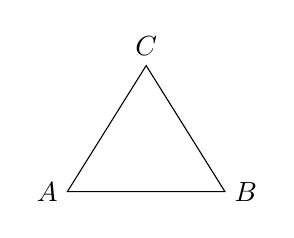
\begin{tikzpicture}
            \draw (-1, 0) node[left] {$A$} -- (1, 0) node[right] {$B$} -- (0, 1.6) node[above] {$C$} -- cycle;
        \end{tikzpicture}
    \end{center}

    Then since $A$ and $B$ don't know each other and at least two of them know each other, then there are three ways we can draw these arrows: 

    \begin{center}
        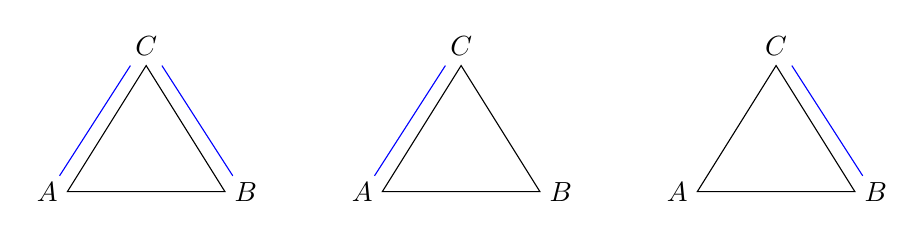
\begin{tikzpicture}
            \draw[blue, -] (-5.1, 0.2)  -- (-4.2, 1.6);
            \draw[blue, -] (-2.9, 0.2) -- (-3.8, 1.6);
            \draw (-5, 0) node[left] {$A$} -- (-3, 0) node[right] {$B$} -- (-4, 1.6) node[above] {$C$} -- cycle;

            \draw[blue, -] (-1.1, 0.2) -- (-0.2, 1.6);
            \draw (-1, 0) node[left] {$A$} -- (1, 0) node[right] {$B$} -- (0, 1.6) node[above] {$C$} -- cycle;
            \draw[blue, -] (5.1, 0.2) -- (4.2, 1.6);
            \draw (3, 0) node[left] {$A$} -- (5, 0) node[right] {$B$} -- (4, 1.6) node[above] {$C$} -- cycle;
        \end{tikzpicture}
    \end{center}

    Now we form two groups, based on whether $A$ or $B$ knows $C$. If both of them know $C$, then put $C$ in either group. There are 43 people at this party, so to split them into two groups, then it follows that at least one of the two groups will have at least 22 people. This is because $21 + 22 = 43$, so no matter how we divide these two groups at least one will always have larger than 22 elements within it.
\end{solution}

\end{document}